%<<< TeX hoá bằng MyLT >>>
%<<< https://www.facebook.com/mylt2018 >>>

\documentclass[12pt,a4paper]{article}
\usepackage{amsmath,amssymb,fancyhdr}
\usepackage{tkz-euclide}
\usepackage{tikz,tikz-3dplot,tkz-tab}
\usetikzlibrary{arrows,intersections,angles,quotes,shapes.geometric}
\usepackage[top=1.5cm, bottom=2cm, left=2cm, right=1.5cm]{geometry}
\usepackage[solcolor]{ex_test}
\usetikzlibrary{calc,patterns,intersections}
\newcommand{\heva}[1]{\left\{\begin{aligned}#1\end{aligned}\right.}
\pagestyle{fancy}
\fancyhf{}
\renewcommand{\headrulewidth}{0pt}
\renewcommand{\footrulewidth}{0pt}
\begin{document}

%Trái
\begin{minipage}[b]{4.5cm}
\centerline{\footnotesize\textbf{BỘ GIÁO DỤC VÀ ĐÀO TẠO}}
\centerline{\footnotesize\textbf{ĐỀ THAM KHẢO}}
\centerline{\footnotesize(\textit{Đề thi có \pageref{mylt}\ trang})}
\end{minipage}\hspace{1cm}
%Phải
\begin{minipage}[b]{12cm}
\centerline{\footnotesize\textbf{KỲ THI TỐT NGHIỆP THPT TỪ NĂM 2025}}
\centerline{\footnotesize\textbf{MÔN: TOÁN}}
\centerline{\footnotesize\textit{Thời gian làm bài: 90\ phút, không kể thời gian phát đề}}
\end{minipage}\\
%Họ tên
\begin{minipage}[b]{10cm}
\vspace{6pt}\textbf{Họ và tên thí sinh: }{\tiny\dotfill}\\
\textbf{Số báo danh: }{\tiny\dotfill}
\end{minipage}\hfill
\begin{minipage}[b]{7.5cm}
\flushright\fbox{\bf \LaTeX\,hoá - MyLT}
\end{minipage}\hfill
%chân trang
\rfoot{Trang \thepage/\pageref{mylt}}
\noindent\textbf{PHẦN I.} Thí sinh trả lời từ câu 1 đến câu 12. Mỗi câu hỏi thí sinh chỉ chọn một phương án.
\Opensolutionfile{ans}[ansMyLTTN]
\begin{ex}%Câu 1
Nguyên hàm của hàm số $f(x)=e^x$ là
\choice
{$\dfrac{e^{x+1}}{x+1}+C$}
{\True $e^x+C$}
{$\dfrac{e^x}{x}+C$}
{$x \cdot e^{x-1}+C$}
\end{ex}

\begin{ex}%Câu 2
Cho hàm số $y=f(x)$ liên tục, nhận giá trị dương trên đoạn $[a ; b]$. Xét hình phẳng $(H)$ giới hạn bởi đồ thị hàm số $y=f(x)$, trục hoành và hai đường thẳng $x=a, x=b$. Khối tròn xoay được tạo thành khi quay hình phẳng $(H)$ quanh trục $O x$ có thể tích là
\choice
{$V=\pi \displaystyle\int\limits_a^b|f(x)| \mathrm{\,d}x$}
{$V=\pi^2 \displaystyle\int\limits_a^b f(x) \mathrm{\,d}x$}
{$V=\pi^2 \displaystyle\int\limits_a^b[f(x)]^2 \mathrm{\,d}x$}
{\True $V=\pi \displaystyle\int\limits_a^b[f(x)]^2 \mathrm{\,d}x$}
\end{ex}

\begin{ex}%Câu 3
Hai mẫu số liệu ghép nhóm $M_1, M_2$ có bảng tần số ghép nhóm như sau
\begin{center}
$M_1 \quad$\begin{tabular}{|c|c|c|c|c|c|}
\hline Nhóm &{$[8 ; 10)$}&{$[10 ; 12)$}&{$[12 ; 14)$}&{$[14 ; 16)$}&{$[16 ; 18)$}\\
\hline Tần số & 3 & 4 & 8 & 6 & 4 \\
\hline
\end{tabular}\\
$M_2\quad$\begin{tabular}{|c|c|c|c|c|c|}
\hline Nhóm &{$[8 ; 10)$}&{$[10 ; 12)$}&{$[12 ; 14)$}&{$[14 ; 16)$}&{$[16 ; 18)$}\\
\hline Tần số & 6 & 8 & 16 & 12 & 8 \\
\hline
\end{tabular}
\end{center}
Gọi $s_1, s_2$ lần lượt là độ lệch chuẩn của mẫu số liệu ghép nhóm $M_1, M_2$. Phát biểu nào sau đây là \textbf{đúng}?
\choice
{\True $s_1=s_2$}
{$s_1=2 s_2$}
{$2 s_1=s_2$}
{$4 s_1=s_2$}
\end{ex}

\begin{ex}%Câu 4
Trong không gian với hệ trục tọa độ $O x y z$, phương trình của đường thẳng đi qua điểm $M(1 ;-3 ; 5)$ và có một vectơ chỉ phương $\vec{u}(2 ;-1 ; 1)$ là
\choice
{$\dfrac{x-1}{2}=\dfrac{y-3}{-1}=\dfrac{z-5}{1}$}
{$\dfrac{x-1}{2}=\dfrac{y-3}{-1}=\dfrac{z+5}{1}$}
{\True $\dfrac{x-1}{2}=\dfrac{y+3}{-1}=\dfrac{z-5}{1}$}
{$\dfrac{x+1}{2}=\dfrac{y+3}{-1}=\dfrac{z-5}{1}$}
\end{ex}

\begin{ex}%Câu 5
\immini{
Cho hàm số $y=\dfrac{a x+b}{c x+d}(c \neq 0, a d-b c+0)$ có đồ thị như hình vẽ bên. Tiệm cận ngang của đồ thị hàm số là
\choice
{$x=-1$}
{\True $y=\dfrac{1}{2}$}
{$y=-1$}
{$x=\dfrac{1}{2}$}
}{
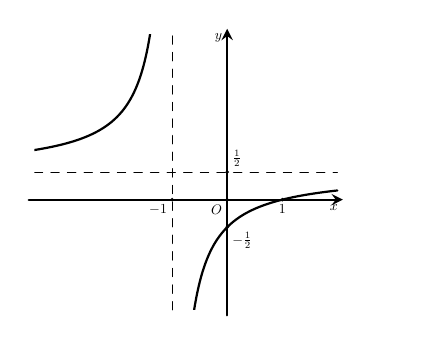
\begin{tikzpicture}[line join=round, line cap=round,>=stealth,thick,scale=0.7]
\tikzset{every node/.style={scale=0.5}}
\draw[->] (-3.6,0)--(2.1,0) node[below left] {$x$};
\draw[->] (0,-2.1)--(0,3.1) node[below left] {$y$};
\foreach \i in {-1,1,0}{\fill (\i,0) circle(1pt);}
\foreach \i in {-0.5,0.5}{\fill (0,\i) circle(1pt);}
\path (0,0) node [below left] {$O$};
\path(-1,0) node [below left] {$-1$};
\path(1,0) node [below] {$1$};
\path(0,-0.5) node [below right] {$-\frac{1}{2}$};
\path(0,0.5) node [above right] {$\frac{1}{2}$};
\draw[dashed,thin] (-0.99,-2)--(-0.99,3);
\begin{scope}
\clip (-3.5,-2) rectangle (3,3);
\draw[samples=200,domain=-3.5:-1.01,smooth,variable=\x] plot (\x,{(1*(\x)+-1)/(2*(\x)+2)});
\draw[samples=200,domain=-0.99:2,smooth,variable=\x] plot (\x,{(1*(\x)+-1)/(2*(\x)+2)});
\draw[dashed,thin] (-3.5,1/2)--(2,1/2);
\end{scope}
\end{tikzpicture}
}
\end{ex}

\begin{ex}%Câu 6
Tập nghiệm của bất phương trình $\log_2(x-1)<3$ là
\choice
{\True $(1 ; 9)$}
{$(-\infty ; 9)$}
{$(9 ;+\infty)$}
{$(1 ; 7)$}
\end{ex}

\begin{ex}%Câu 7
Trong không gian với hệ trục tọa độ $O x y z$, cho mặt phẳng $(P)$ có phương trình $x-3 y-z+8=0$. Vectơ nào sau đây là một vectơ pháp tuyến của mặt phẳng $(P)$?
\choice
{$\overrightarrow{n_1}(1 ;-3 ; 1)$}
{\True $\overrightarrow{n_2}(1 ;-3 ;-1)$}
{$\overrightarrow{n_3}(1 ;-3 ; 8)$}
{$\vec{n}_4(1 ; 3 ; 8)$}
\end{ex}

\begin{ex}%Câu 8
Cho hình chóp $S \cdot A B C D$ có đáy $A B C D$ là hình chữ nhật và $S A \perp(A B C D)$. Mặt phẳng nào sau đây vuông góc với mặt phẳng $(A B C D)$?
\choice
{\True $(S A B)$}
{$(S B C)$}
{$(S C D)$}
{$(S B D)$}
\end{ex}

\begin{ex}%Câu 9
Nghiệm của phương trình $2^x=6$ là
\choice
{$x=\log_6 2$}
{$x=3$}
{$x=4$}
{\True $x=\log_2 6$}
\end{ex}

\begin{ex}%Câu 10
Cấp số cộng $\left(u_n\right)$ có $u_1=1$ và $u_2=3$. Số hạng $u_5$ của cấp số cộng là
\choice
{$5$}
{$7$}
{\True $9$}
{$11$}
\end{ex}

\begin{ex}%Câu 11
\immini{
Cho hình hộp $A B C D \cdot A^{\prime}B^{\prime}C^{\prime}D^{\prime}(\operatorname{minh}$ họa như hình bên). Phát biểu nào sau đây là \textbf{đúng}?
\choice
{$\overrightarrow{A B}+\overrightarrow{B B^{\prime}}+\overrightarrow{B^{\prime}A^{\prime}}=\overrightarrow{A C^{\prime}}$}
{$\overrightarrow{A B}+\overrightarrow{B C^{\prime}}+\overrightarrow{C^{\prime}D^{\prime}}=\overrightarrow{A C^{\prime}}$}
{$\overrightarrow{A B}+\overrightarrow{A C}+\overrightarrow{A A^{\prime}}=\overrightarrow{A C^{\prime}}$}
{\True $\overrightarrow{A B}+\overrightarrow{A A^{\prime}}+\overrightarrow{A D}=\overrightarrow{A C^{\prime}}$}
}{
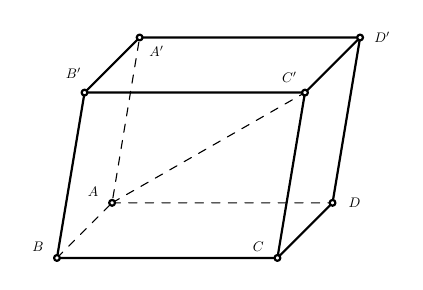
\begin{tikzpicture}[line join=round, line cap=round,thick,scale=0.7]
\def\ccao{3}
\coordinate (A) at (0,0);
\coordinate (B) at (-1,-1);
\coordinate (D) at (4,0);
\coordinate (C) at ($(B)+(D)-(A)$);
\coordinate (A') at ($(A)+(0.5,\ccao)$);
\coordinate (B') at ($(B)+(0.5,\ccao)$);
\coordinate (C') at ($(C)+(0.5,\ccao)$);
\coordinate (D') at ($(D)+(0.5,\ccao)$);
\draw(A')--(B')--(C')--(D')--cycle (B')--(B)--(C)--(C') (C)--(D)--(D');
\draw[dashed,thin](B)--(A)--(A') (A)--(C') (A)--(D);
\foreach \i/\g in {A/150,B/150,C/150,D/0,A'/-40,B'/120,C'/135,D'/0}{\draw[fill=white](\i) circle (1.5pt) ($(\i)+(\g:4mm)$) node[scale=0.5]{$\i$};}
\end{tikzpicture}
}
\end{ex}

\begin{ex}%Câu 12
\immini{
Cho hàm số có đồ thị như hình vẽ bên. Hàm số đã cho đồng biến trên khoảng nào sau đây?
\choice
{$(-\infty ;-1)$}
{$(-\infty ; 1)$}
{\True $(-1 ; 1)$}
{$(1 ;+\infty)$}
}{
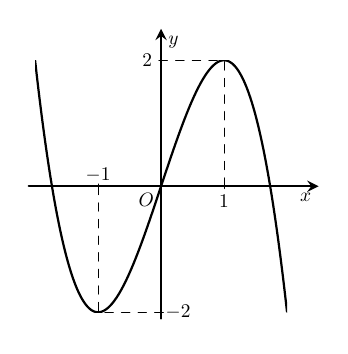
\begin{tikzpicture}[line join=round, line cap=round,>=stealth,thick,scale=0.8]
\tikzset{every node/.style={scale=0.7}}
\draw[->] (-2.1,0)--(2.5,0) node[below left] {$x$};
\draw[->] (0,-2.1)--(0,2.5) node[below right] {$y$};
\draw (0,0) node [below left] {$O$};
\draw[dashed,thin](-1,0)--(-1,-2)--(0,-2);
\draw[dashed,thin](1,0)--(1,2)--(0,2);
\draw[thin] (-1,1pt)--(-1,-1pt) node [above] {$-1$};
\draw[thin] (1,1pt)--(1,-1pt) node [below] {$1$};
\draw[thin] (1pt,-2)--(-1pt,-2) node [right] {$-2$};
\draw[thin] (1pt,2)--(-1pt,2) node [left] {$2$};
\begin{scope}
\clip (-2,-2) rectangle (2,2);
\draw[samples=200,domain=-2:2,smooth,variable=\x] plot (\x,{-1*((\x)^3)+0*((\x)^2)+3*(\x)+0});
\end{scope}
\end{tikzpicture}
}
\end{ex}
\Closesolutionfile{ans}

\noindent\textbf{PHẦN II.} Thí sinh trả lời từ câu 1 đến câu 4. Mỗi ý \textbf{a), b), c), d)} ở mỗi câu hỏi, thí sinh chọn đúng hoặc sai.
\setcounter{ex}{0}
\Opensolutionfile{ans}[ansMyLTTF]
\begin{ex}%Câu 13
Cho hàm số $f(x)=2 \cos x+x$.
\choiceTFt
{\True $f(0)=2 ; f\left(\dfrac{\pi}{2}\right)=\dfrac{\pi}{2}$}
{Đạo hàm của hàm số đã cho là $f^{\prime}(x)=2 \sin x+1$}
{\True Nghiệm của phương trình $f^{\prime}(x)=0$ trên đoạn $\left[0 ; \dfrac{\pi}{2}\right]$ là $\dfrac{\pi}{6}$}
{\True Giá trị lớn nhất của $f(x)$ trên đoạn $\left[0 ; \dfrac{\pi}{2}\right]$ là $\sqrt{3}+\dfrac{\pi}{6}$}
\loigiai{
	\begin{itemchoice}
		\itemch Đúng.$f(0)=2$ ; $f(\dfrac{\pi}{2})=\dfrac{\pi}{2}$
		\itemch Sai . $f' (x)=-2\sin x+1$
		\itemch Đúng. $f'(x)=0\Leftrightarrow\sin x=\dfrac{1}{2}\Leftrightarrow\left[\begin{aligned}
			& x=\dfrac{\pi}{6}+k2\pi\\ 
			& x=\dfrac{5\pi}{6}+k2\pi\\ 
		\end{aligned}\right.(k\in\mathbb{Z})$ .Dễ thấy nghiệm trên đoạn $[0;\dfrac{\pi}{2}]$ là $\dfrac{\pi}{6}$ .
		\itemch Đúng .$f(0)=2,f\left(\dfrac{\pi}{2}\right)=\dfrac{\pi}{2},f\left(\dfrac{\pi}{6}\right)=\dfrac{\pi}{6}+\sqrt{3}$ nên giá trị lớn nhất của $f(x)$ trên đoạn $[0;\dfrac{\pi}{2}]$ là $\dfrac{\pi}{6}+\sqrt{3}$ .
	\end{itemchoice}
}
\end{ex}

\begin{ex}%Câu 14
Một người điều khiển ô tô đang ở đường dẫn muốn nhập làn vào đường cao tốc. Khi ô tô cách điểm nhập làn 200 m , tốc độ của ô tô là $36 \mathrm{~km}/ \mathrm{h}$. Hai giây sau đó, ô tô bắt đầu tăng tốc với tốc độ $v(t)=a t+b(a, b \in \mathbb{R}, a>0)$, trong đó $t$ là thời gian tính bằng giây kể từ khi bắt đầu tăng tốc. Biết rằng ô tô nhập làn cao tốc sau 12 giây và duy trì sự tăng tốc trong 24 giây kể từ khi bắt đầu tăng tốc.
\choiceTFt
{\True Quãng đường ô tô đi được từ khi bắt đầu tăng tốc đến khi nhập làn là 180 m }
{\True Giá trị của $b$ là 10 }
{Quãng đường $S(t)$ (đơn vị: mét) mà ô tô đi được trong thời gian $t$ giây $(0 \leq t \leq 24)$ kể từ khi tăng tốc được tính theo công thức $S(t)=\displaystyle\int\limits_0^{24}v(t) \mathrm{,d}t$}
{Sau 24 giây kể từ khi tăng tốc, tốc độ của ô tô không vượt quá tốc độ tối đa cho phép là $100 \mathrm{~km}/ \mathrm{h}$}
\loigiai{
	\begin{itemchoice}
		\itemch Đúng. Ta có $36~km/h=10~m/s\Rightarrow s(2)=20~m$ . Vậy quãng đường ô tô đi được từ khi bắt đầu tăng tốc đến khi nhập làn là $200-20=180~m$
		\itemch Đúng. Trước khi tăng tốc vận tốc của xe là $10~m/s$ .
		\itemch Sai . Vì $S(t)=\displaystyle\int_0^{24}v(t) dt$ là quãng đường đi được trong $24$ giây chứ không phải trong $t$ giây.
		\itemch Sai. Ta có $180=\displaystyle\int\limits_0^{12}{\left(at+10\right)dt\Rightarrow v(t)=\dfrac{5}{6}}t+10\Rightarrow v(24)=30~m/s=108~km/h$ .
	\end{itemchoice}
}
\end{ex}

\begin{ex}%Câu 15
Trước khi đưa một loại sản phẩm ra thị trường, người ta đã phỏng vấn ngẫu nhiên 200 khách hàng về sản phẩm đó. Kết quả thống kê như sau: có 105 người trả lời ``sẽ mua''; có 95 người trả lời ``không mua''. Kinh nghiệm cho thấy tỉ lệ khách hàng thực sự sẽ mua sản phẩm tương ứng với những cách trả lời ``sẽ mua'' và ``không mua'' lần lượt là $70 \%$ và $30 \%$.
Gọi $A$ là biến cố ``Người được phỏng vấn thực sự sẽ mua sản phẩm''.
Gọi $B$ là biến cố ``Người được phỏng vấn trả lời sẽ mua sản phẩm''.
\choiceTFt
{\True Xác suất $P(B)=\dfrac{21}{40}$ và $P(\bar{B})=\dfrac{19}{40}$}
{Xác suất có điều kiện $P(A \mid B)=0,3$}
{\True Xác suất $P(A)=0,51$}
{Trong số những người được phỏng vấn thực sự sẽ mua sản phẩm có $70 \%$ người đã trả lời ``sẽ mua'' khi được phỏng vấn (kết quả tính theo phần trăm được làm tròn đến hàng đơn vị)}
\loigiai{
	\begin{itemchoice}
		\itemch Đúng . $P(B)=\dfrac{105}{200}=\dfrac{21}{40}$ ,$P(\overline{B})=\dfrac{19}{40}$
		\itemch Sai .$P(A|B)=\dfrac{P(A\cap B)}{P(B)}=\dfrac{0,7.\dfrac{21}{40}}{\dfrac{21}{40}}=0,7$
		\itemch Đúng . $P(A)=\dfrac{0,7.105+0,3.95}{200}=0,51$
		\itemch Sai . Số người thực sự mua là: $0,7.105+0,3,95=102$ ,phần trăm số người trả lời sẽ mua là $\dfrac{0,7.105}{102}.100\approx 72\%$
	\end{itemchoice}
}
\end{ex}

\begin{ex}%Câu 16
\immini{
Các thiên thạch có đường kính lớn hơn $140 m$ và có thể lại gần Trái Đất ở khoảng cách nhỏ hơn 7500000 km được coi là những vật thể có khả năng va chạm gây nguy hiểm cho Trái Đất. Để theo dõi những thiên thạch này, người ta đã thiết lập các trạm quan sát các vật thể bay gần Trái Đất. Giả sử có một hệ thống quan sát có khả năng theo dõi các vật thể ở độ cao không vượt quá 6600 km so với mực nước biển. Coi Trái Đất là khối cầu có bán kính 6400 km . Chọn hệ trục tọa độ $O x y z$ trong không gian có gốc $O$ tại tâm Trái Đất và đơn vị độ dài trên mỗi trục tọa độ là 1000 km . Một thiên thạch (coi như một hạt) chuyển động với tốc độ không đổi theo một đường thẳng từ điểm $M(6 ; 20 ; 0)$ đến điểm $N(-6 ;-12 ; 16)$
}{
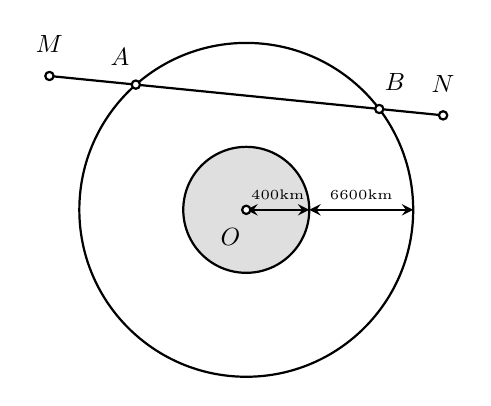
\begin{tikzpicture}[line join=round, line cap=round,>=stealth,thick]
\coordinate (O) at (0,0);
\coordinate (M) at (-2.5,1.7);
\coordinate (N) at (2.5,1.2);
\draw[name path=dto](O) circle (2.12cm);
\draw[fill=gray!25] (O) circle (0.8 cm);
\draw[name path=MN] (M)--(N);
\path [name intersections={of=MN and dto,by={B,A}}];
\draw[<->] (O)--(0.8,0) node [above ,sloped,pos=0.5] {\tiny 400km};
\draw[<->] (0.8,0)--(2.12,0) node [above ,sloped,pos=0.5] {\tiny 6600km};
\foreach \i/\g in {A/120,B/60,M/90,N/90,O/-120}{\draw[fill=white](\i) circle (1.5pt) ($(\i)+(\g:4mm)$) node[scale=0.9]{$\i$};}
\end{tikzpicture}
}
\choiceTFt
{\True Đường thẳng $M N$ có phương trình tham số là $\left\{\begin{aligned}&x=6+3t \\ &y=20+8t\\&z=-4 t\end{aligned}\right.$, $(t \in \mathbb{R})$}
{Vị trí đầu tiên thiên thạch di chuyển vào phạm vi theo dõi của hệ thống quan sát là điểm $A(-3 ;-4 ; 12)$}
{\True Khoảng cách giữa vị trí đầu tiên và vị trí cuối cùng mà thiên thạch di chuyển trong phạm vi theo dõi của hệ thống quan sát là 18900 km (kết quả làm tròn đến hàng trăm theo đơn vị ki-lô-mét)}
{\True Nếu thời gian di chuyển của thiên thạch trong phạm vi theo dõi của hệ thống quan sát là 3 phút thì thời gian nó di chuyển từ $M$ đến $N$ là 6 phút}
\loigiai{
	\begin{itemchoice}
		\itemch Đúng .$\overrightarrow{MN}=-4(3;8;-4)$\\
		Suy ra:Đường thẳng $MN$ có phương trình tham số là $\begin{cases}x=6+3t\\ y=20+8t\\ z=-4t\end{cases}$ ($t\in\mathbb{R}$).
		\itemch Sai. Ta có thiên thạch là 1 chất điểm có tâm nằm trên đường $MN$ có bán kính lớn hơn $0,07$ (km).Do vậy thiên thạch nằm trong phạm vi theo dõi thỏa mãn\\
		$\sqrt{\left(6+3t\right)^2+\left(20+8t\right)^2+\left(4t\right)^2}\le 13,00007\Leftrightarrow 89t^2+356t-266,99818\le 0(*)$ nên điểm đầu tiên sẽ không phải điểm A.
		\itemch Đúng. Gọi $t_1,t_2$ lần lượt tương ứng với vị trí đầu tiên, vị trí cuối cùng trong phạm vi theo dõi.\\
		Ta có : $\left\{\begin{aligned}
			&{t_1}+t_2=-\dfrac{356}{89}\\ 
			&{t_1}.t_2=\dfrac{-266,99818}{89}\\ 
		\end{aligned}\right.$ .Khi đó khoảng cách từ điểm đầu đến điểm cuối là\\
		$1000.\sqrt{89\left(t_1-t_2\right)^2}=1000.\sqrt{89\left[\left(t_1+t_2\right)^2-4t_1.t_2\right]}\approx 18900~km$
		\itemch Đúng . Ta có $1000.\sqrt{89\left[\left(t_1+t_2\right)^2-4t_1.t_2\right]}$ km đi hết mất 3 phút, vậy 6 phút thiên thạch đi được $2000.\sqrt{89\left[\left(t_1+t_2\right)^2-4t_1.t_2\right]}\approx 37700=MN$
	\end{itemchoice}
}
\end{ex}
\Closesolutionfile{ans}

\noindent\textbf{PHẦN III.} Thí sinh trả lời từ câu 1 đến câu 6.
\setcounter{ex}{0}
\Opensolutionfile{ans}[ansMyLTSA]
\begin{ex}%Câu 17
Cho hình lăng trụ đứng $A B C . A^{\prime}B^{\prime}C^{\prime}$ có $A B=5, B C=6, C A=7$. Khoảng cách giữa hai đường thẳng $A A^{\prime}$ và $B C$ bằng bao nhiêu? (làm tròn kết quả đến hàng phần mười).
\shortans{$4{,}9$}
\loigiai{
\begin{center}
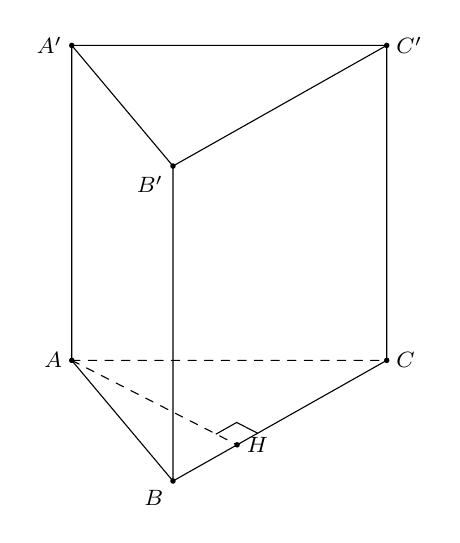
\begin{tikzpicture}[scale=1, font=\footnotesize, line join=round, line cap=round, >=stealth]
	\def\ac{4} \def\ab{2}  \def\h{4}  \def\gocA{50} 
	\coordinate[label=left:$A$] (A) at (0,0);
	\coordinate[label=right:$C$] (C) at (\ac,0);
	\coordinate[label=below left:$B$] (B) at (-\gocA:\ab);
	\coordinate[label=left:$A'$] (A') at ($(A)+(90:\h)$);
	\coordinate[label=below left:$B'$] (B') at ($(B)-(A)+(A')$);
	\coordinate[label=right:$C'$] (C') at ($(C)-(A)+(A')$);
	\draw (A')--(A)--(B)--(C)--(C')--(A')--(B')--(C') (B)--(B');
	\coordinate[label=right:$H$] (H) at ($(B)!0.3!(C)$);
	\draw[dashed] (A)--(C) (A)--(H);
	\draw pic[draw,angle radius=3mm]{right angle=C--H--A};
	\foreach \diem in {A,B,C,A',B',C',H} \fill (\diem)circle(1pt);
\end{tikzpicture}
\end{center}
Ta có:	$d(AA',BC)=AH=\dfrac{2S_{ABC}}{BC}=\dfrac{2\sqrt{9.4.3.2}}{6}\approx 4,9$
	}
\end{ex}

\begin{ex}%Câu 18
\immini{
Một trò chơi điện tử quy định như sau: Có 4 trụ $A, B, C, D$ với số lượng các thử thách trên đường đi giữa các cặp trụ được mô tả trong hình bên. Người chơi xuất phát từ một trụ nào đó, đi qua tất cả các trụ còn lại, mỗi khi đi qua một trụ thì trụ đó sẽ bị phá hủy và không thể quay trở lại trụ đó được nữa, nhưng người chơi vẫn phải trở về trụ ban đầu. Tổng số thử thách của đường đi thoả mãn điều kiện trên nhận giá trị nhỏ nhất là bao nhiêu?
}{
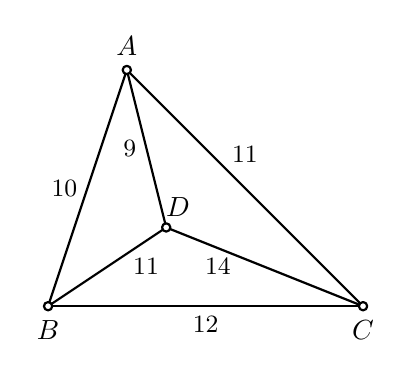
\begin{tikzpicture}[line join=round, line cap=round,thick]
\coordinate (A) at (0,3);
\coordinate (B) at (-1,0);
\coordinate (C) at (3,0);
\coordinate (D) at (0.5,1);
\draw (A)--(B) node [midway,left] {\small 10};
\draw (B)--(C) node [midway,below] {\small 12};
\draw (C)--(A) node [midway,above=2mm] {\small 11};
\draw (D)--(A) node [midway,left] {\small 9};
\draw (D)--(B) node [midway,right=2mm] {\small 11};
\draw (D)--(C) node [midway,left=3mm] {\small 14};
\foreach \i/\g in {A/90,B/-90,C/-90,D/60}{\draw[fill=white](\i) circle (1.5pt) ($(\i)+(\g:3mm)$) node[scale=1]{$\i$};}
\end{tikzpicture}
}
\shortans{43}
\loigiai{
	Xuất phát từ trụ A sẽ có\\ $ABCDA=45,ABDCA=46,ACBDA=43,ACDBA=46,ADBCA=43,ADCBA=45$\\
	Các trường hợp còn lại có được bằng cách thay thế $A\to B,B\to A$ và $A\to C,C\to A$ và $A\to D,D\to A$ .Khi đó tổng số thử thách không thay đổi so với xuất phát từ trụ $A.$\\
	Vậy tổng số thử thách nhỏ nhất là : $43$}
\end{ex}

\begin{ex}%Câu 19
Hệ thống định vị toàn cầu GPS là một hệ thống cho phép xác định vị trí của một vật thể trong không gian. Trong cùng một thời điểm, vị trí của một điểm $M$ trong không gian sẽ được xác định bởi bốn vệ tinh cho trước nhờ các bộ thu phát tín hiệu đặt trên các vệ tinh. Giả sử trong không gian với hệ tọa độ $O x y z$, có bốn vệ tinh lần lượt đặt tại các điểm $A(3 ; 1 ; 0), B(3 ; 6 ; 6)$, $C(4 ; 6 ; 2), D(6 ; 2 ; 14)$; vị trí $M(a ; b ; c)$ thỏa mãn $M A=3, M B=6, M C=5, M D=13$.
Khoảng cách từ điểm $M$ đến điểm $O$ bằng bao nhiêu?
\shortans{3}
\loigiai{
	Ta có:$\left\{\begin{aligned}
		&{a^2}+b^2+c^2-6a-2b=-1\\ 
		&{a^2}+b^2+c^2-6a-12b-12c=-45\\ 
		&{a^2}+b^2+c^2-8a-12b-4c=-31\\ 
		&{a^2}+b^2+c^2-12a-4b-28c=-67\\ 
	\end{aligned}\right.\Leftrightarrow\left\{\begin{aligned}
		&-10b-12c=-44\\ 
		&-2a-10b-4c=-30\\ 
		&-6a-2b-28c=-66\\ 
	\end{aligned}\right.\Leftrightarrow\left\{\begin{aligned}
		& a=1\\ 
		& b=2\\ 
		& c=2\\ 
	\end{aligned}\right.$\\
	Vậy $OM=3$}
\end{ex}

\begin{ex}%Câu 20
\immini{
Kiến trúc sư thiết kế một khu sinh hoạt cộng đồng có dạng hình chữ nhật với chiều rộng và chiều dài lần lượt là 60 m và 80 m . Trong đó, phần được tô màu đậm là sân chơi, phần còn lại để trồng hoa. Mỗi phần trồng hoa có đường biên cong là một phần của parabol với đỉnh thuộc một trục đối xứng của hình chữ nhật và khoảng cách từ đỉnh đó đến trung điểm cạnh tương ứng của hình chữ nhật bằng $20 m$ (xem hình minh họa). Diện tích của phần sân chơi là bao nhiêu mét vuông?
}{
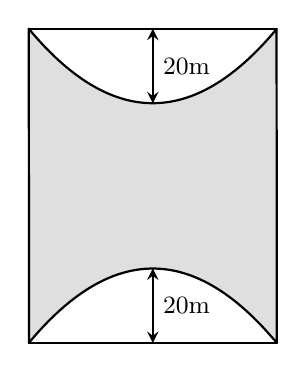
\begin{tikzpicture}[line join=round, line cap=round,thick,xscale=1.5,yscale=0.6,>=stealth,scale=0.7]
\draw[<->] (0,2.5)--(0,4.75) node [midway,right] {\small 20m};
\draw[<->] (0,-2.5)--(0,-4.75) node [midway,right] {\small 20m};
\draw[fill=gray!25] plot[samples=200,domain=-1.5:1.5,smooth,variable=\x] (\x,{(\x)^2+2.5})--plot[samples=200,domain=1.5:-1.5,smooth,variable=\x] (\x,{-(\x)^2-2.5})--cycle;
\draw(-1.5,4.75)--(1.5,4.75) (-1.5,-4.75)--(1.5,-4.75);
\end{tikzpicture}
}
\shortans{3200}
\loigiai{
	\begin{center}
	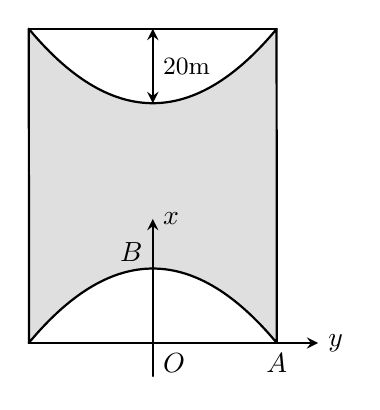
\begin{tikzpicture}[line join=round, line cap=round,thick,xscale=1.5,yscale=0.6,>=stealth,scale=0.7]
		\draw[<->] (0,2.5)--(0,4.75) node [midway,right] {\small 20m};
		\draw[fill=gray!25] plot[samples=200,domain=-1.5:1.5,smooth,variable=\x] (\x,{(\x)^2+2.5})--plot[samples=200,domain=1.5:-1.5,smooth,variable=\x] (\x,{-(\x)^2-2.5})--cycle;
		\draw(-1.5,4.75)--(1.5,4.75) (-1.5,-4.75)--(1.5,-4.75);
		\draw[->] (0,-5.75)--(0,-1) node [right] {$x$};
		\draw[->] (-1.5,-4.75)--(2,-4.75) node [right] {$y$};
		\draw (0,-4.75) node[below right]{$O$};
		\draw (1.5,-4.75) node[below ]{$A$};
		\draw (0,-2) node[ left]{$B$};
	\end{tikzpicture}
	\end{center}
	Gắn hệ trục $Oxy$ như hình vẽ. Ta có $A(30;0),B(0;20)\Rightarrow (P):y=-\dfrac{1}{45}{x^2}+20$\\
	Khi đó diện tích phần parabol là: $4\displaystyle\int\limits_0^{30}{\left(-\dfrac{1}{45}{x^2}+20\right)}dx=1600~(m^2)$\\
	Vậy diện tích phần sân chơi là: $60.80-1600=3200~(m^2)$}
\end{ex}

\begin{ex}%Câu 21
Một doanh nghiệp dự định sản xuất không quá 500 sản phẩm. Nếu doanh nghiệp sản xuất $x$ sản phẩm $(1 \leq x \leq 500)$ thì doanh thu nhận được khi bán hết số sản phẩm đó là $F(x)=x^3-1999 x^2+1001000 x+250000$ (đồng), trong khi chi phí sản xuất bình quân cho một sản phẩm là $G(x)=x+1000+\dfrac{250000}{x}$ (đồng). Doanh nghiệp cần sản xuất bao nhiêu sản phẩm để lợi nhuận thu được là lớn nhất?
\shortans{333}
\loigiai{
	Lợi nhuận thu được khi sản xuất và bán đi $x$ sản phẩm là giá trị của hàm số:\\
	$f(x)=F(x)-x.G(x)=x^3-2000x^2+1000000x$\\
	$f'(x)=3x^2-4000x+1000000$\\
	Bảng biến thiên:
	\begin{center}
		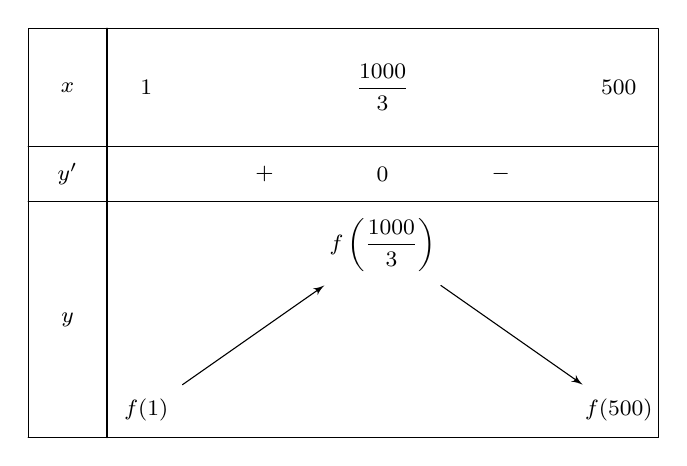
\begin{tikzpicture}[scale=1, font=\footnotesize, line join=round, line cap=round, >=stealth]
			\tkzTabInit[nocadre=false,lgt=1,espcl=3,deltacl=0.5]
			{$x$/1.5 ,$y'$/.7,$y$/3}
			{$1$ , $\dfrac{1000}{3}$ , $500$}
			\tkzTabLine{ , + , $0$ , - , }
			\tkzTabVar{-/$f(1)$ , +/$f\left(\dfrac{1000}{3}\right)$ , -/$f(500)$}
		\end{tikzpicture}
	\end{center}
	Vậy đề có lợi nhuận cao nhất thì cần sản xuất $333$ sản phẩm}
\end{ex}

\begin{ex}%Câu 22
Có hai chiếc hộp, hộp I có 6 quả bóng màu đỏ và 4 quả bóng màu vàng, hộp II có 7 quả bóng màu đỏ và 3 quả bóng màu vàng, các quả bóng có cùng kích thước và khối lượng. Lấy ngẫu nhiên một quả bóng từ hộp I bỏ vào hộp II. Sau đó, lấy ra ngẩu nhiên một quả bóng từ hộp II. Tính xác suất để quả bóng được lấy ra từ hộp II là quả bóng được chuyển từ hộp I sang, biết rằng quả bóng đó có màu đỏ (làm tròn kết quả đến hàng phần trăm).
\shortans{0,08}
\loigiai{
	Công việc được hoàn thành bởi 2 hành động liên tiếp, lấy 1 quả ở hộp I bỏ vào hộp II, sau đó lấy 1 quả ở hộp II.Nên $n(\Omega)=110$\\
	Gọi A:” lấy được quả màu đỏ ở hộp II” $n(A)=6.8+4.7=76$\\
	B:”lấy 1 quả ở hộp II được quả ở hộp I chuyển qua” $n(B)=10.1=10\Rightarrow n(A\cap B)=6$\\
	Ta có: $P(B|A)=\dfrac{P(A\cap B)}{P(A)}=\dfrac{6}{76}\approx 0,08$}
\end{ex}
\Closesolutionfile{ans}
\label{mylt}
\centerline{\rule[0.5ex]{2cm}{1pt} HẾT \rule[0.5ex]{2cm}{1pt}}

\newpage
\setcounter{page}{1}
\rfoot{Trang \thepage}
\begin{center}
\bf ĐÁP ÁN PHẦN I
\inputansbox[1]{6}{ansMyLTTN}
\end{center}
\begin{center}
\bf ĐÁP ÁN PHẦN II
\end{center}
\inputansbox[2]{2}{ansMyLTTF}
\begin{center}
\bf ĐÁP ÁN PHẦN III
\end{center}
\inputansbox[3]{3}{ansMyLTSA}
\end{document}